\chapter{Experiments}

% Short introduction such as: this chapter describes how the tests should be
% conducted, explain thorougly the scheduler script, gathered data etc.
\section{Proposed workflow and methodology}

In order to obtain the details of how system-level physical measurement
estimates energy consumption by a component (such as a CPU or a GPU)
during an application execution, several steps must be taken:

\begin{enumerate}
    \item Exclusive reservation of the entire computational node.
    \item Observation of the disk consumption and network usage before and
    during tests.
    \item Monitoring of the CPUs and GPUs utilization before and during tests.
    \item Running the benchmark kernels on an abstract processor only.
    Abstract processor comprises of the multicore CPU processor consisting
    of a certain number of physical cores and DRAM\@.
    \item Gathering of the power measurements.
    \item Verification of the accuracy and reliability of the software
    measurements tools, based on ground truth results.
\end{enumerate}

One of the notable mentions that could be done in order to reduce the amount
of uncertain power draw measurements done by the background components is
setting the fans to full speed. This solution have a potential of reducing
power draw fluctuations, especially during higher workloads, i\. e\. when
running benchmarks kernels utilizing maximum amount of GPUs or running Hybrid
configuration, where power draw of the entire nodes are very high. This could
not be implemented, however, as the administrator of the department's servers
stated, that interference in servers fans could be crucial for the nodes
stability.

\textbf{For Intel RAPL / NVIDIA Management Library:}
\begin{enumerate}
    \item Obtain base power of idle CPUs / GPUs.
    \item Obtain execution time of benchmark application.
    \item Obtain total energy consumption of the CPUs / GPUs during tests.
    \item Calculate dynamic energy consumption by subtracting base energy from
    total energy used during run.
\end{enumerate}

\textbf{For Yokotool:}
\begin{enumerate}
    \item Obtain base power of idle CPUs.
    \item Obtain execution time of benchmark application.
    \item Obtain total energy consumption of the CPUs during tests.
    \item Calculate dynamic energy consumption by subtracting base power from
    total energy used during run
\end{enumerate}

\newpage

In addition to the main experiments workflow, another methodology must be
adapted $-$ the data collection methodology. In order for the results to be
properly comparable, several point have to be met:
\begin{enumerate}
    \item Tests environment must be identical in every case, to eliminate
    discrepancy of the results.
    \item The results of the power draw reading must be properly compared for
    the device only measurements (Intel RAPL / NVML) and the measurements of
    the entire node (Yokotool).
    \item Experiments should be conducted on different nodes that utilizes
    different hardware, in order to state repeatability of tests. [TO BE REDACTED]
    \item Experiments should be conducted, using different benchmark kernels
    or application, to remove the possibility of bias of the results, due to
    poor diversification of test cases. [TO BE REDACTED]
    \item Test runs must be repeated many times.
\end{enumerate}

\section{Working environment $-$ servers details}

[PLACEHOLDER]
% Describe more thoroughly the nodes: CPUs, GPUs, RAM, PSUs, PM connection etc

\section{Main tests}

\subsection{Overview on the scheduler script}

In order to automate the experiments, an entire scheduler script had to be
created. Its has two main tasks: first is to store the information about the
configurations and run the benchmarks according to the presets. The second
is to run the measurements softwares and save all the results in the ordered
manner.

Both of these goals are reached by using dictionaries with key-value pairs.
That created a~tree-like dependencies between the corresponding layers of
configurations. Finally, that solution works for both choosing the right
config and providing the path to save measurements.


2. Section that run CPUs benchmarks, GPUs benchmarks, perf, nvml, yoko
3. Functions that check if the benchmarks are still running
4. Function that cleans-up every process after tests

\newpage

\subsection{Main automation function $-$ scheduler()}

% NOTE TO SELF: Make sure this chart belongs to this section

The entire scheduler script consists of classes and functions that are
explicitly designated for their purposes in the code. Overview of them is
as follows:

\begin{itemize}
    \item \textbf{class `Config'} $-$ Contains all the informations about the servers,
    devices, implementations, benchmarks and configurations, handles the
    relations between them and provides correct pathes to the corresponding
    measurements directories.
    \item \textbf{class `Benchmark'} $-$ Defines functions responsible for
    executing CPUs and GPUs benchmarks, as well as the measurements
    softwares: Linux Perf, NVIDIA Management Library and Yokotool
    \item \textbf{class `Execution'} $-$ This class contains functions tasked with
    calling the benchmark kernels and checking their status, if they are still
    running, for the purpose of ending the measurements. Since the
    measurements softwares are highly dependent on benchmarks being run, they
    are executed directly from the \emph{main\@()} function and
    the \emph{Execution} class only has the functions tasked with the proper
    termination of them.
    \item \textbf{function `scheduler\@()'} $-$ This major function triggers
    secondary functions from \emph{Execution} class and watched their status.
    \item \textbf{function `main\@()'} $-$ Runs every configuration
    sequentially, based on the lists of presets. Additionally, repeats every
    ten times in order to achieve repeatability of the experiments.
\end{itemize}

In order to visualize the entire workflow of the scheduler, as well as the 
workings of the individual processes, two charts has been created:
\begin{itemize}
    \item \textbf{General Flowchart} $-$ This chart
    (\textbf{Fig. \ref{fig:general_flowchart}}) describes the relations
    between the currently used configurations and the instructions executed
    based on those conditions.
    \item \textbf{Processes Flowchart} $-$ This chart
    (\textbf{Fig. \ref{fig:processes_flowchart}}) shows the working priciples of the
    \emph{runner\@()} subfunction, which shows the benchmarks and measurements
    softwares are started on a~high level of abstraction.
\end{itemize}

\newpage

\begin{figure}[hbtp!]
    \centering
    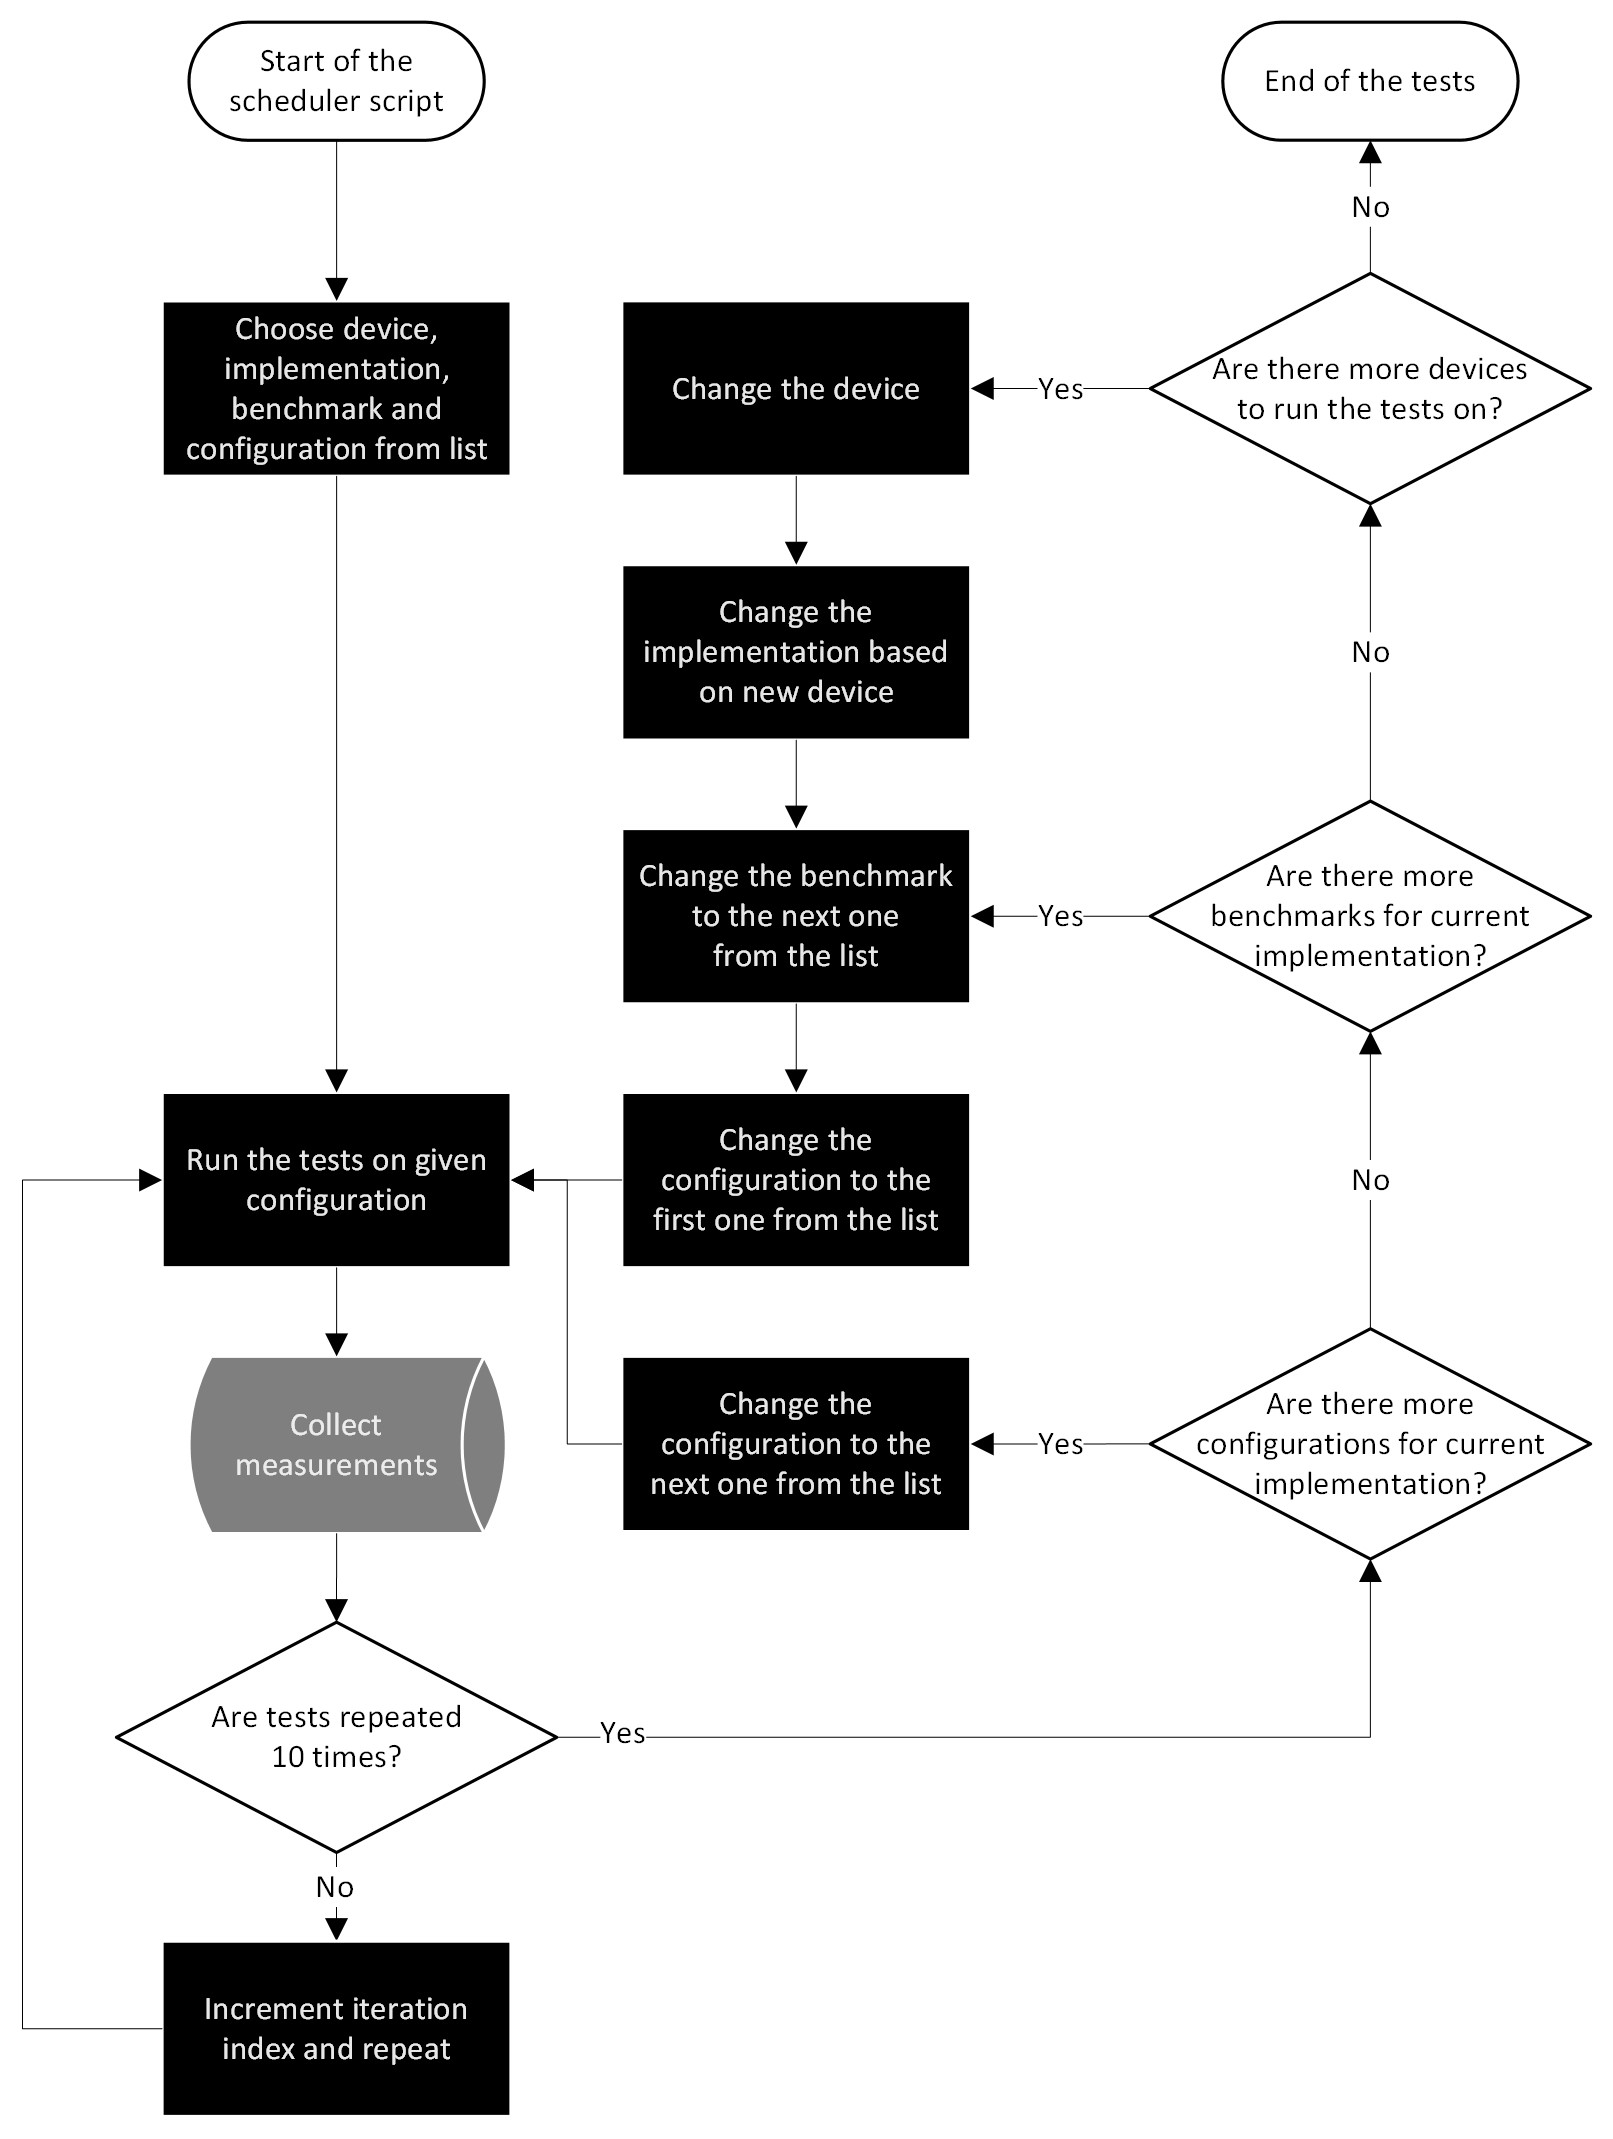
\includegraphics{general_flowchart}
    \caption{General Flowchart}~\label{fig:general_flowchart}
\end{figure}

\begin{figure}[hbtp!]
    \centering
    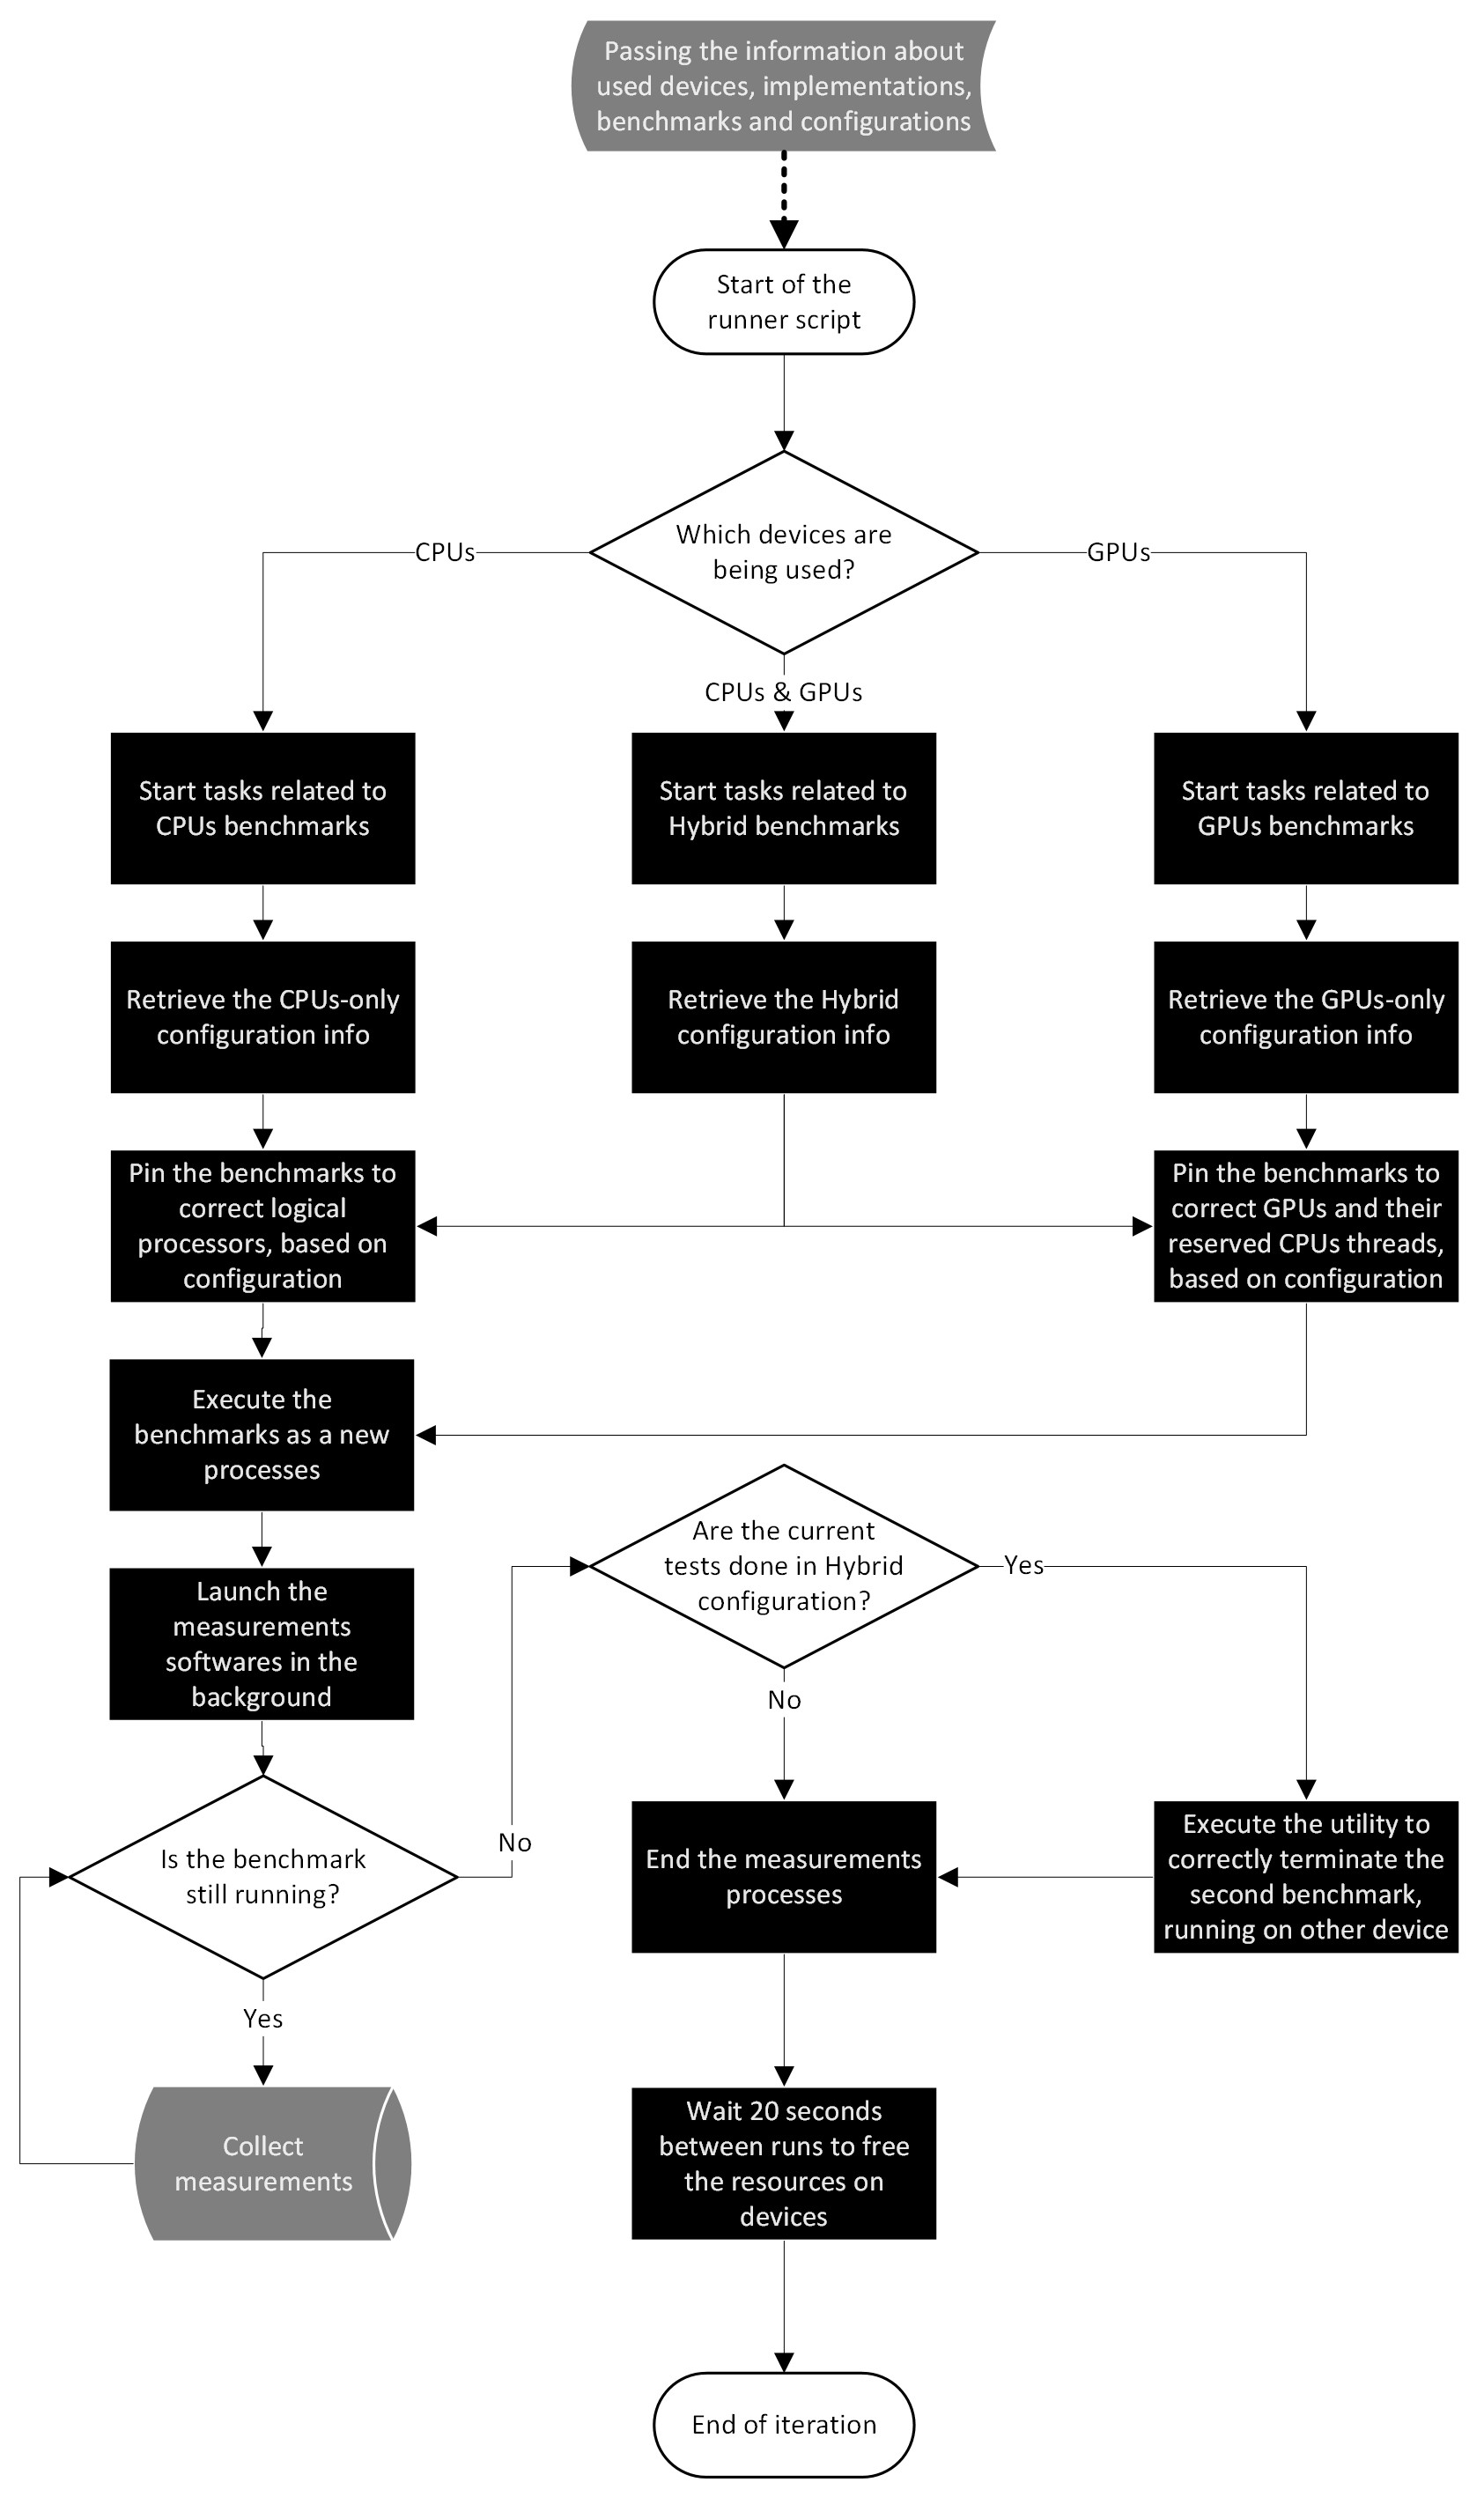
\includegraphics{processes_flowchart.jpeg}
    \caption{Processes Flowchart}~\label{fig:processes_flowchart}
\end{figure}

\newpage

\subsection{Threads pinning and kernels execution $-$ cpu\_benchmark()}

This function is responsible of executing CPUs benchmarks, based on the
given configuration. It creates a separate processes by utilizing the
Python \emph{subprocess} module. 

\begin{lstlisting}[language=Python]
    cpu_benchmark = subprocess.Popen(
        [
            "taskset --cpu-list <T> <P> <B> > /dev/null 2>&1"
        ],
        shell=True,
    )
\end{lstlisting}

Here is an explanation of every part of the command:

\begin{itemize}
    \item \textbf{cpu\_benchmark} $-$ text
    \item \textbf{subprocess.Popen} $-$ text
    \item \textbf{taskset} $-$ This command is used to set or retrieve the
    CPU affinity of a running process given its pid, or to launch a new
    command with a given CPU affinity.
    \item \textbf{--cpu-list} $-$ This option interprets mask as numerical
    list of processors instead of a bitmask. Numbers are separated by
    commas and may include ranges. For example: 0,5,8-11.
    \item Variables that dynamically changes based on the configurations:
    \begin{conditions}
        \textbf{T} & Logical processors indexes \\
        \textbf{P} & Specified absolute path to the correct measurements folder \\
        \textbf{B} & Currently used benchmark kernel \\
    \end{conditions}
    \item \textbf{\textgreater~/dev/null 2\textgreater\&1} $-$
    Redirecting \emph{stderr} containing error messages from the
    executed command or script to \emph{stdout} to the output of the
    command. Both are, in fact, redirected then to the so-called
    \emph{null device}. The result of that action is suppression of all
    messages printed by the benchmark kernels. It is useful when
    collecting logs from the terminal, that is running the entire
    scheduler script, without unnecessary messages.
    \item \textbf{shell=True} $-$ text
\end{itemize}

Finally, the function returns the PID of newly created process
as an integer value. It is done for the purpose of terminating the
benchmark in a Hybrid configuration.

\subsection{GPUs and threads management $-$ gpu\_benchmark\@()}

This function consists of two parts: first part is responsible for executing
the Horovod-Python benchmark and the second part is responsible for running
the OMP-CUDA benchmark.

\begin{lstlisting}[language=Python]
    gpu_benchmark = subprocess.Popen(
        [
            "mpirun -np <N> --map-by socket -x NCCL_DEBUG=INFO \
            python3 <P>+"Xception.py"
        ],
        shell=True
    )
\end{lstlisting}

\subsection{Measurements with Yokotool software $-$ yoko\@()}

\subsection{Measurements with Linux Perf software $-$ perf\@()}

\subsection{Measurements with NVML handling function $-$ nvml\@()}

\subsection{Cleanup of measurements daemons}

\subsection{Termination of benchmarks in Hybrid configuration}

% psutil

[PLACEHOLDER]
% Put the charts and plots of received measurements

\newpage

\section{Analysis of the results and discussion}

\begin{table}[hbt!]
    \rowcolors{1}{Lavender!80!gray}{white}
    \centering
    \caption{sanna.kask, CPUs, OMP-CPP, bt.C, 1 CPU [POWER DRAW ONLY!!!]}\label{tbl:sanna.kask_CPUs_OMP-CPP_bt.C}
    \setlength{\tabcolsep}{5mm}
    \begin{tblr}{
        % {|l|c|c|c|c|},
        % hlines,
        vlines,
        row{1}={font=\bfseries,halign=c,bg=lightgray!30},
        row{7-8} = {bg = lightgray!20}
        }
    \hline
        & \SetCell[c=4]{c} 1 CPU  \\
    \hline
        Results from 10 runs                                    & 1 Thread  & 5 Threads & 10 Threads    & 20 Threads \\
    \hline
        {Avg. Exec\@. time [s]}                                 & 1054.795  & 216.315   & 114.315       & 101.372 \\
    \hline
        {Std\@. dev\@. of time [-]}                             & 0.966     & 0.243     & 0.121         & 0.158 \\
    \hline
        {(Yokogawa) \\ Avg\@. power draw [W]}                   & 379.962   & 402.881   & 432.171       & 445.752 \\
    \hline
        {(Yokogawa) \\ Std\@. dev\@. of avg\@. power draw [-]}  & 0.605     & 0.225     & 0.382         & 1.007 \\
    \hline
        {(CPU\@: 0) \\ Avg\@. power draw [W]}                   & 33.717    & 51.274    & 70.433        & 77.958 \\
    \hline
        {(CPU\@: 0) \\ Std\@. dev\@. of avg\@. power draw [-]}  & 0.102     & 0.13      & 0.085         & 0.089 \\
    \hline
        {(CPU\@: 1) \\ Avg\@. power draw [W]}                   & 28.98     & 28.887    & 28.871        & 28.874 \\
    \hline
        {(CPU\@: 1) \\ Std\@. dev\@. of avg\@. power draw [-]}  & 0.125     & 0.062     & 0.067         & 0.055 \\
    \hline
        {(GPU\@: 0) \\ Avg\@. power draw [W]}                   & 21.755    & 21.673    & 21.604        & 21.634 \\
    \hline
        {(GPU\@: 0) \\ Std\@. dev\@. of avg\@. power draw [-]}  & 0.343     & 0.061     & 0.2           & 0.05 \\
    \hline
        {(GPU\@: 1) \\ Avg\@. power draw [W]}                   & 25.522    & 25.534    & 25.516        & 25.524 \\
    \hline
        {(GPU\@: 1) \\ Std\@. dev\@. of avg\@. power draw [-]}  & 0.023     & 0.032     & 0.052         & 0.029 \\
    \hline
        {(GPU\@: 2) \\ Avg\@. power draw [W]}                   & \\
    \hline
        {(GPU\@: 2) \\ Std\@. dev\@. of avg\@. power draw [-]}  & \\
    \hline
        {(GPU\@: 3) \\ Avg\@. power draw [W]}                   & \\
    \hline
        {(GPU\@: 3) \\ Std\@. dev\@. of avg\@. power draw [-]}  & \\
    \hline
        {(GPU\@: 4) \\ Avg\@. power draw [W]}                   & \\
    \hline
        {(GPU\@: 4) \\ Std\@. dev\@. of avg\@. power draw [-]}  & \\
    \hline
        {(GPU\@: 5) \\ Avg\@. power draw [W]}                   & \\
    \hline
        {(GPU\@: 5) \\ Std\@. dev\@. of avg\@. power draw [-]}  & \\
    \hline
        {(GPU\@: 6) \\ Avg\@. power draw [W]}                   & \\
    \hline
        {(GPU\@: 6) \\ Std\@. dev\@. of avg\@. power draw [-]}  & \\
    \hline
        {(GPU\@: 7) \\ Avg\@. power draw [W]}                   & \\
    \hline
        {(GPU\@: 7) \\ Std\@. dev\@. of avg\@. power draw [-]}  & \\
    \hline
    \end{tblr}
\end{table}


% \begin{table}[hbt!]
%     % \centering
%     % \small
%     \caption{sanna.kask, CPUs, OMP-CPP, bt.C [POWER DRAW ONLY!!!]}\label{tbl:sanna.kask_CPUs_OMP-CPP_bt.C}
%     \begin{tblr}{|c|c|c|c|c|c|c|c|c|}
%     \hline
%         & \SetCell[c=4]{c} 1 CPU & & & & \SetCell[c=4]{c} 2 CPUs \\
%     \hline
%         (10 runs) & 1 Thread & 5 Threads & 10 Threads & 20 Threads & 2 Threads & 10 Threads & 20 Threads & 40 Threads \\
%     \hline
%         {Avg. \\ Exec\@. time [s]} & \\
%     \hline
%         {Std\@. dev\@. \\ of time [-]} & \\
%     \hline
%         {(Yokogawa) Avg\@. \\ power draw [W]} & \\
%     \hline
%         {(Yokogawa) Std\@. \\ dev\@. of avg\@. \\ power draw [-]} & \\
%     \hline
%         {(CPU:0) Avg\@. \\ power draw [W]} & \\
%     \hline
%         {(CPU:0) Std\@. dev\@. \\ of avg\@. \\ power draw [-]} & \\
%     \hline
%         {(CPU:1) Avg\@. \\ power draw [W]} & \\
%     \hline
%         {(CPU:1) Std\@. dev\@. \\ of avg\@. \\ power draw  [-]} & \\
%     \hline
%     \end{tblr}
% \end{table}

[PLACEHOLDER]
% Put the analysis of the received data, according to Dr. Czarnul